%! alt Two horizontal parallel lines 12 apart, with A and B on the lower line and AB = 24. On the upper line, D and D' are the two points at distance 13 from A, 5 to the right and 5 to the left of the point above A, and C and C' are the two points at distance 20 from B, 16 to the right and 16 to the left of the point above B. The trapezium ABCD is outlined and shaded, with the perpendicular of length 12 from D to AB dashed. Dashed segments join A to D' and B to C', the other positions of D and C. The four possible top sides are DC = 35, D'C = 45, DC' = 3 and D'C' = 13.
%! after_paragraph 1
%! scale 1/6
% The shared preamble of every Cevian figure. pipeline/figures turns these colours into theme-aware paint,
% and refuses any other colour, so draw only with them:
%   figink (lines and labels), figaux (construction lines), figaccent (the object the argument turns on),
%   figtint and figaccenttint (light fills).
\documentclass[border=1.5pt]{standalone}
\usepackage{tkz-euclide}
\definecolor{figink}{RGB}{0,0,0}
\definecolor{figaux}{RGB}{85,85,85}
\definecolor{figaccent}{RGB}{192,57,43}
\definecolor{figtint}{RGB}{221,221,221}
\definecolor{figaccenttint}{RGB}{245,213,208}
% tkz-euclide's defaults draw circles, compasses and marks in 50% grey and fill points with a tint.
\makeatletter
\def\tkz@otherlinecolor{figink}
\def\tkz@euc@circlecolor{figink}
\def\tkz@euc@compasscolor{figink}
\def\tkz@euc@mkcolor{figink}
\def\tkz@mk@fill{figink}
\def\tkz@euc@pointfillcolor{figink}
\makeatother
\tkzSetUpLine[color=figink,line width=.7pt]
\tkzSetUpArc[color=figink,line width=.7pt]
\tkzSetUpCompass[color=figink,line width=.5pt]
\tkzSetUpPoint[color=figink,fill=figink,size=3.1pt]
\tikzset{
  every picture/.style={line cap=round,line join=round,color=figink},
  circle style/.append style={color=figink,line width=.7pt},
  aux/.style={color=figaux,line width=.45pt,dash pattern=on 2.6pt off 2pt},
  key/.style={color=figaccent,line width=1pt},
  mk/.style={color=figink,line width=.5pt},
  lbl/.style={color=figink,inner sep=2.2pt},
  len/.style={color=figink,inner sep=1.5pt,font=\small},
}

\begin{document}
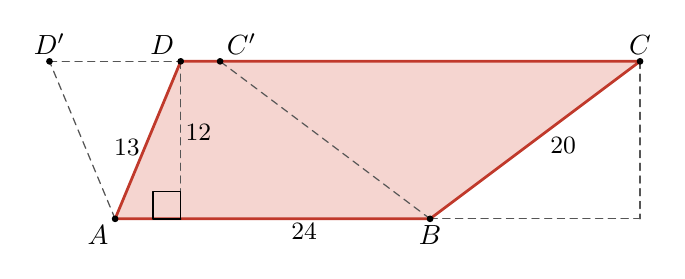
\begin{tikzpicture}
\tkzDefPoint(0.0,0.0){A} %! A = (0, 0)
\tkzDefPoint(4.0000000,0.0){B} %! B = (24, 0)
\tkzDefPoint(0.83333333,2.0000000){D} %! D = (5, 12)
\tkzDefPoint(-0.83333333,2.0000000){Dp} %! Dp = (-5, 12)
\tkzDefPoint(6.6666667,2.0000000){C} %! C = (40, 12)
\tkzDefPoint(1.3333333,2.0000000){Cp} %! Cp = (8, 12)
\tkzDefPoint(0.83333333,0.0){H} %! H = (5, 0)
\tkzDefPoint(6.6666667,0.0){K} %! K = (40, 0)
%! fact dist(A, B) == 24
%! fact dist(A, D) == 13
%! fact dist(A, Dp) == 13
%! fact dist(B, C) == 20
%! fact dist(B, Cp) == 20
%! fact dist(D, H) == 12
%! fact perp(D, H, A, B)
%! fact parallel(A, B, D, C)
%! fact collinear(Dp, D, C)
%! fact collinear(Cp, D, C)
%! fact collinear(K, A, B)
%! fact dist(A, H) == 5
%! fact dist(B, K) == 16
%! fact dist(D, C) == 35
%! fact dist(Dp, C) == 45
%! fact dist(D, Cp) == 3
%! fact dist(Dp, Cp) == 13
\tkzFillPolygon[color=figaccenttint](A,B,C,D)
\tkzDrawSegment[aux](B,K)
\tkzDrawSegment[aux](C,K)
\tkzDrawSegment[aux](D,H)
\tkzDrawSegment[aux](Dp,D)
\tkzDrawSegment[aux](A,Dp)
\tkzDrawSegment[aux](B,Cp)
\tkzDrawPolygon[key](A,B,C,D)
\tkzMarkRightAngle[size=.35,mk](A,H,D)
\tkzDrawPoints(A,B,C,D,Cp,Dp)
\tkzLabelPoint[below left,lbl](A){$A$}
\tkzLabelPoint[below,lbl](B){$B$}
\tkzLabelPoint[above,lbl](C){$C$}
\tkzLabelPoint[above left,lbl](D){$D$}
\tkzLabelPoint[above right,lbl](Cp){$C'$}
\tkzLabelPoint[above,lbl](Dp){$D'$}
\tkzLabelSegment[below,pos=.6,len](A,B){$24$}
\tkzLabelSegment[right,pos=.45,len](D,H){$12$}
\tkzLabelSegment[below right,pos=.55,len](B,C){$20$}
\tkzLabelSegment[left,pos=.45,len](A,D){$13$}
\end{tikzpicture}
\end{document}
